\section{Measurements}

First thing to do with the measurements is to subtract the bias from the sensor data. For this, the sensor has been put on a flat surface and recorded 500 samples along 10 seconds. The values have been averaged to obtain the bias (see table \ref{tab:bias}) and later subtracted to any following Kalman Filtering.

\begin{table}[h]
    \centering
    \begin{tabular}{|c|c|c|c|}
    \hline
    Sensor bias & x & y & z\\ \hline
    Accelerometer $(m/s^2)$ & 0.817012 & -0.045973 & 10.379578 \\ \hline
    Gyroscope ($\degree/s$) & -0.0170254 &  0.0262836 & -0.0076507 \\
    \hline
\end{tabular}
    \caption{Sensor measurement bias measured on flat surface.}
    \label{tab:bias}
\end{table}

To test the setup, the sensor has been handheld and rotated first 45 degrees roll in each direction, and then 45 degrees pitch in each direction. In figure \ref{fig:sensor_data} we can see the raw data from the accelerometer and the gyroscope.

\begin{figure}[h]
\centering
\begin{subfigure}[b]{0.45\textwidth}
    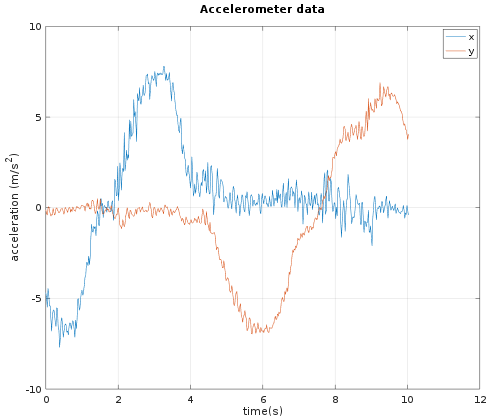
\includegraphics[width=\textwidth]{figures/acc_data.png}
    \caption{Accelerometer measurements}
    \label{fig:acc_data}
\end{subfigure}
\begin{subfigure}[b]{0.45\textwidth}
    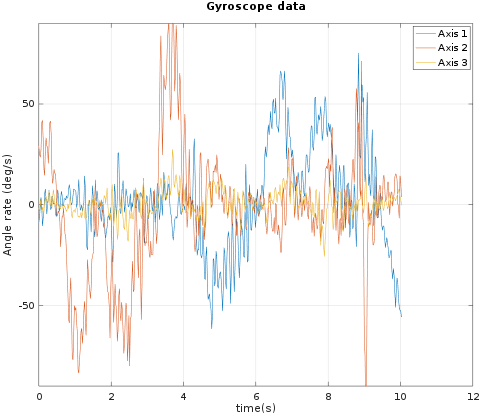
\includegraphics[width=\textwidth]{figures/gyro_data.png}
    \caption{Gyroscope measurements}
    \label{fig:gyro_data}
\end{subfigure}
\caption{Raw Sensor data}
\label{fig:sensor_data}
\end{figure}

Then we apply Extended Kalman Filter to the data and obtain the results in figure \ref{fig:kalman_results}. Figure \ref{fig:acc_attitude} is the estimated attitude computed directly from the accelerometer data using equation \ref{eq:meas}. Figure \ref{fig:kalman_results} is the estimated attitude obtained from the output of the Extended Kalman Filter. We can see it is much smoother than the attitude from the accelerometer data.

\begin{figure}[h]
\centering
\begin{subfigure}[b]{0.45\textwidth}
    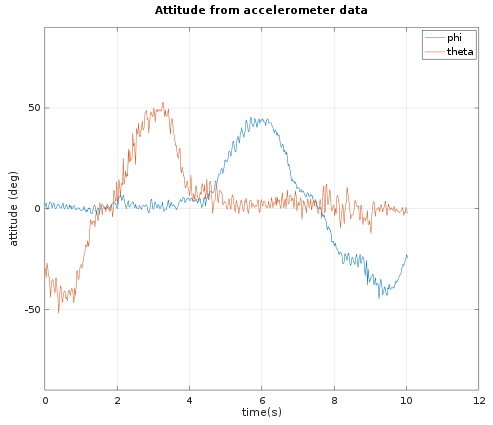
\includegraphics[width=\textwidth]{figures/acc_attitude.png}
    \caption{Attitude from accelerometer.}
    \label{fig:acc_attitude}
\end{subfigure}
\begin{subfigure}[b]{0.45\textwidth}
    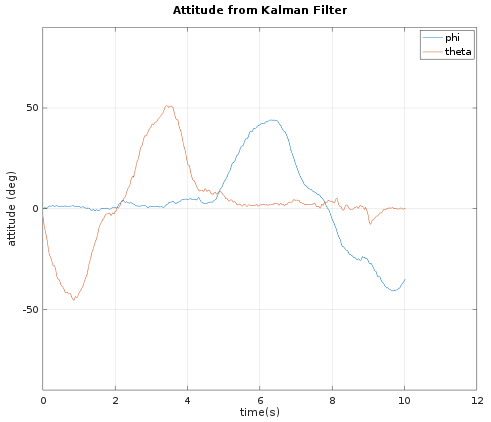
\includegraphics[width=\textwidth]{figures/attitude_kalman.png}
    \caption{Attitude from Kalman Filter}
    \label{fig:attitude_kalman}
\end{subfigure}
\caption{Attitude estimation}
\label{fig:kalman_results}
\end{figure}
